%==============================================================================
%  Homework template  --  999 Controls
%
%  To reuse for the next assignment:
%    1. copy this folder,  2. edit the METADATA block below,
%    3. edit the SOLUTIONS section,  4. run  `make`.
%
%  Build:  make          (regenerates code output, then builds main.pdf)
%          make clean    (removes build artifacts)
%==============================================================================
\documentclass[11pt,letterpaper]{article}

%------------------------------- METADATA -------------------------------------
\newcommand{\hwcourse}{EE 999 --- Introduction to Control Systems}
\newcommand{\hwcourseshort}{EE 999}  % running head, keep it short
\newcommand{\hwtitle}{Homework 7}
\newcommand{\hwauthor}{Patrick Gordon}
\newcommand{\hwdate}{\today}
\newcommand{\hwdue}{Due Wednesday, November 4, 2026}
%------------------------------------------------------------------------------

\usepackage[T1]{fontenc}
\usepackage[utf8]{inputenc}
\usepackage{textcomp}
\usepackage[letterpaper,margin=1in,headheight=14pt]{geometry}
\usepackage{amsmath,amssymb}
\usepackage{cancel}
\usepackage{array}
\usepackage{graphicx}
\usepackage[american]{circuitikz}
\usepackage{xcolor}
\usepackage{listings}
\usepackage{fancyhdr}
\usepackage{inconsolata}
\usepackage{pdflscape}
\usepackage{float}
\usepackage[hidelinks]{hyperref}

%--- page furniture -----------------------------------------------------------
\pagestyle{fancy}
\fancyhf{}
\lhead{\hwauthor}
\chead{\hwtitle}
\rhead{\hwcourseshort}
\cfoot{\thepage}

%--- listing styles -----------------------------------------------------------
\definecolor{codebg}{HTML}{F7F7F4}
\definecolor{outbg}{HTML}{FCFCFC}
\definecolor{rule}{HTML}{C8C8C0}
\definecolor{kw}{HTML}{1C4FA1}
\definecolor{cmt}{HTML}{6A7A5A}
\definecolor{str}{HTML}{A0522D}

\lstdefinestyle{mcode}{
  language=Octave,
  basicstyle=\ttfamily\footnotesize,
  keywordstyle=\color{kw}\bfseries,
  commentstyle=\color{cmt}\itshape,
  stringstyle=\color{str},
  backgroundcolor=\color{codebg},
  frame=single,
  rulecolor=\color{rule},
  framesep=6pt,
  numbers=left,
  numberstyle=\ttfamily\scriptsize\color{gray},
  numbersep=8pt,
  showstringspaces=false,
  breaklines=true,
  columns=fullflexible,
  keepspaces=true,
  upquote=true,
}

\lstdefinestyle{moutput}{
  basicstyle=\ttfamily\footnotesize,
  backgroundcolor=\color{outbg},
  frame=single,
  rulecolor=\color{rule},
  framesep=6pt,
  showstringspaces=false,
  breaklines=true,
  columns=fullflexible,
  keepspaces=true,
  upquote=true,
}

%--- structure helpers --------------------------------------------------------
% \problem{1.1b}{Optional title}
\newcommand{\problem}[2]{%
  \bigskip
  \noindent{\large\bfseries Problem #1}%
  \ifx\relax#2\relax\else\ {\large --- #2}\fi
  \par\nobreak\vspace{2pt}\hrule\vspace{8pt}\nobreak
}

% \caplabel{Code}{hw_02_A.m}
\newcommand{\caplabel}[2]{%
  \par\nobreak\vspace{6pt}\nobreak
  \noindent{\small\bfseries #1}\ {\small\ttfamily \detokenize{#2}}%
  \par\nobreak\vspace{2pt}\nobreak
}

% \matlabcode{hw_02_A.m}  -- source listing pulled straight from the .m file
\newcommand{\matlabcode}[1]{%
  \caplabel{Code:}{#1}%
  \lstinputlisting[style=mcode]{#1}%
}

% \codeoutput{output/hw_02_A.txt} -- console output captured by the Makefile
\newcommand{\codeoutput}[1]{%
  \caplabel{Output:}{#1}%
  \IfFileExists{#1}{\lstinputlisting[style=moutput]{#1}}{\missing{#1}{run \texttt{make} to generate it}}%
}

% \answerfigure[width]{figures/foo.pdf}{Caption}  -- placeholder if not exported
% yet. Any format graphicx reads works: pdf, png, jpg.
% A script that plots is exported by the Makefile to figures/<script>.pdf, so
% \answerfigure{figures/hw_02_F.pdf}{...} is how a plotted answer is included.
% The optional argument is the printed width, default the full text width.
% Give a scan or screenshot a smaller one so it is not blown up past its own
% resolution:  \answerfigure[0.8\linewidth]{figures/some_scan.png}{...}
\newcommand{\answerfigure}[3][\linewidth]{%
  \begin{figure}[H]
    \centering
    \IfFileExists{#2}{\includegraphics[width=#1]{#2}}{\missing{#2}{export it, see README}}
    \caption{#3}
  \end{figure}%
}

% \splane{G_1(s)}  -- an empty s-plane grid to sketch poles (x) and zeros (o)
% on by hand. One unit per square, Re from -10 to 3 and Im from -4 to 4.
% \splane[5]{G_2(s)} instead centres the origin, both axes running -5 to 5.
\newcommand{\splane}[2][]{%
  \ifx\relax#1\relax
    \def\spxmin{-10}\def\spxmax{3}\def\spymax{4}\def\spxlabels{-10,-8,...,2}\def\spylabels{-4,-2,2,4}\def\spscale{1}%
  \else
    \def\spxmin{-#1}\def\spxmax{#1}\def\spymax{#1}\def\spxlabels{-#1,...,-1,1,2,...,#1}\def\spylabels{-#1,...,-1,1,2,...,#1}\def\spscale{0.85}%
  \fi
  \begin{figure}[H]
    \centering
    \begin{tikzpicture}[scale=\spscale]
      \draw[gray!30, thin] (\spxmin,-\spymax) grid (\spxmax,\spymax);
      \draw[->, thick] (\spxmin-0.3,0) -- (\spxmax+0.4,0) node[right] {$\mathrm{Re}$};
      \draw[->, thick] (0,-\spymax-0.3) -- (0,\spymax+0.4) node[above] {$\mathrm{Im}$};
      \foreach \x in \spxlabels
        \node[below, font=\scriptsize, fill=white, inner sep=1pt] at (\x,-0.05) {$\x$};
      \foreach \y in \spylabels
        \node[left, font=\scriptsize, fill=white, inner sep=1pt] at (-0.05,\y) {$\y j$};
    \end{tikzpicture}
    \caption{Pole-zero sketch of $#2$.}
  \end{figure}%
}

%--- tables -------------------------------------------------------------------
% Centred paragraph column, so a description column wraps instead of running
% off the page:  \begin{tabular}{|c|P{0.5\linewidth}|}
\newcolumntype{P}[1]{>{\centering\arraybackslash}p{#1}}

% \begin{symboltable}{Signal}{Caption}  -- the symbol / units / description
% table used to define the variables of a problem. The first argument is the
% heading of the left column (Signal, Parameter, State, ...); leave the second
% empty for no caption.
%
%   \begin{symboltable}{Signal}{}
%     \sym{x(t)}{m}{Position of tire center}
%     \sym{r(t)}{m}{Road height (depends on $v_{car}(t)$)}
%   \end{symboltable}
%
% \sym puts its first argument in math mode and brackets the units, so write
% \sym{x(t)}{m}{...}, not \sym{$x(t)$}{[m]}{...}. Anything already math -- a
% subscript, a fraction -- goes in the description as usual: $\frac{1}{4}$.
%
% The optional argument is the width of the description column, for a table
% whose descriptions are much longer or much shorter than average:
%   \begin{symboltable}[0.35\linewidth]{Parameter}{}
\newcommand{\sym}[3]{$#1$ & [#2] & #3 \\ \hline}
\newenvironment{symboltable}[3][0.45\linewidth]{%
  \def\symtabcap{#3}%
  \begin{table}[H]
  \centering
  \renewcommand{\arraystretch}{1.4}
  \begin{tabular}{|c|c|P{#1}|}
  \hline
  #2 & Units & Description \\ \hline\hline
}{%
  \end{tabular}
  \ifx\symtabcap\empty\else\caption{\symtabcap}\fi
  \end{table}%
}

% \begin{answertable}{|c|c|c|}{Caption} -- any other table. Same placement and
% captioning as \answerfigure, but you write the rows yourself:
%
%   \begin{answertable}{|c|P{0.5\linewidth}|}{Pole locations.}
%     \hline
%     Pole & Behaviour \\ \hline\hline
%     $s=-2$ & decays in half a second \\ \hline
%   \end{answertable}
\newenvironment{answertable}[2]{%
  \def\anstabcap{#2}%
  \begin{table}[H]
  \centering
  \renewcommand{\arraystretch}{1.4}
  \begin{tabular}{#1}
}{%
  \end{tabular}
  \ifx\anstabcap\empty\else\caption{\anstabcap}\fi
  \end{table}%
}

% \begin{termtable}{4}{Caption} -- collect like powers of $s$ when multiplying
% out a characteristic polynomial (or any other expansion). The argument is the
% highest power; the columns and the $s^4 \dots s^0$ header are generated from
% it, so changing the degree is a one-character edit. Leave the second argument
% empty for no caption.
%
% Cells are already in math mode: write m_1m_2, not $m_1m_2$. One row per factor
% you multiplied out, one column per power; leave a cell empty where that factor
% contributes nothing to that power. Rows end with \\, like any tabular.
%
%   \begin{termtable}{4}{Terms of the characteristic polynomial.}
%     m_1m_2 & m_1b & m_1k_s       & bk_s       & k_s(k_s+k_w) \\
%            & m_2b & m_2(k_s+k_w) & b(k_s+k_w) &              \\
%            &      & -b^2         & -bk_s      & -k_s^2
%   \end{termtable}
%
% M is a centred column that is always in math mode. It uses \( \) rather than
% $ $ so that an empty cell stays empty -- a bare $$ would start display math.
\newcolumntype{M}{>{\(}c<{\)}}
\makeatletter
\newcount\tt@i
\newcommand{\tt@cols}{}
\newcommand{\tt@head}{}
\newcommand{\tt@build}[1]{%
  \def\tt@cols{}\def\tt@head{}%
  \tt@i=#1\relax
  \@whilenum\tt@i>\m@ne\do{%
    \edef\tt@cols{\tt@cols M}%
    \ifx\tt@head\@empty
      \edef\tt@head{s^{\the\tt@i}}%
    \else
      \edef\tt@head{\tt@head & s^{\the\tt@i}}%
    \fi
    \advance\tt@i\m@ne
  }%
}
\newenvironment{termtable}[2]{%
  \def\tt@cap{#2}%
  \tt@build{#1}%
  \begin{table}[H]%
  \centering
  \setlength{\tabcolsep}{12pt}%
  \renewcommand{\arraystretch}{1.3}%
  \edef\@tempa{\noexpand\begin{tabular}{\tt@cols}}\@tempa
  \tt@head \\ \hline
}{%
  \end{tabular}
  \ifx\tt@cap\@empty\else\caption{\tt@cap}\fi
  \end{table}%
}
\makeatother

% wideproblem environment -- a problem on its own landscape page, centred.
% Use for diagrams much wider than they are tall, where a portrait page would
% shrink the labels below readable size:
%   \begin{wideproblem}{1.1b}{Title}
%     \answerfigure{figures/x.pdf}{Caption}
%   \end{wideproblem}
\newenvironment{wideproblem}[2]{%
  \begin{landscape}%
    \problem{#1}{#2}%
    \vspace*{\fill}%
}{%
    \vspace*{\fill}%
  \end{landscape}%
}

% \prompt{What special property does b*d have?} -- restate the question
\newcommand{\prompt}[1]{%
  \noindent\textit{#1}\par\vspace{6pt}%
}

% \answer{...}  -- written answer. Leave the body empty for a visible
% placeholder box; fill it in and the box is replaced by the prose.
\newcommand{\answer}[1]{%
  \ifx\relax#1\relax\todo{write the answer here}\else#1\fi
  \par\vspace{4pt}%
}

\newcommand{\todo}[1]{%
  \fbox{\parbox{0.9\linewidth}{\centering\vspace{10pt}\rmfamily\itshape\small
    #1\vspace{10pt}}}%
}

\newcommand{\missing}[2]{%
  \fbox{\parbox{0.9\linewidth}{\centering\vspace{10pt}\ttfamily\small
    missing: \detokenize{#1}\\[4pt]\rmfamily\itshape #2\vspace{10pt}}}%
}


%==============================================================================
\begin{document}

\begin{center}
  {\LARGE\bfseries \hwtitle}\\[4pt]
  {\large \hwcourse}\\[8pt]
  {\hwauthor} \quad\textbullet\quad {\hwdate}\\[4pt]
  {\small\itshape \hwdue}
\end{center}
\vspace{6pt}\hrule

%------------------------------------------------------------------------------
%  SOLUTIONS
%------------------------------------------------------------------------------

\clearpage
\problem{1}{Review questions 4.1 and 4.2}
\prompt{4.1 Give three advantages of feedback in control.}
\answer{
    Feedback can:
    \begin{itemize}
      \item reduce the steady state error inherent to a system
      \item reduce the impact of disturbances to a system
      \item provide stability to unstable systems
    \end{itemize}
}

\prompt{4.2 Give two disadvantages of feedback in control.}
\answer{
    Feedback typically requires:
    \begin{itemize}
        \item more logical complexity
        \item physical sensors (cost association)
    \end{itemize}
}

\clearpage
\problem{2}{Text problem 4.6}
\prompt{Consider the DC motor control system with rate (tachometer) feedback shown in Fig.~4.26(a).}
\answerfigure{figures/fig_4_26.png}{Text figure 4.26 (8th Ed.).}

\problem{2.A}{}
\prompt{Find values for $K'$ and $k_t'$ so that the system of Fig.~4.26(b) has the same transfer function as the system of Fig.~4.26(a).}
\answer{
\begin{figure}[H]
  \centering
  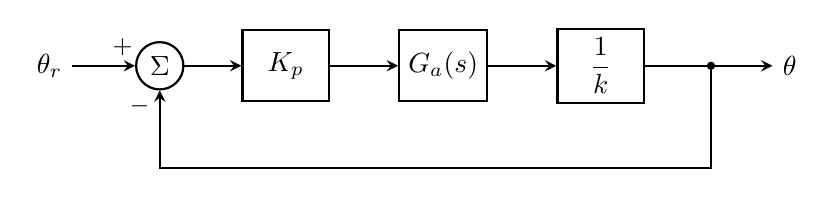
\begin{tikzpicture}[>=stealth, thick,
      blk/.style={draw, minimum height=0.9cm, minimum width=1.1cm},
      sum/.style={draw, circle, inner sep=0pt, minimum size=0.6cm}]
    \node (in)  at (0,0)   {$\theta_r$};
    \node[sum] (s1) at (1.4,0) {$\Sigma$};
    \node[blk] (kp) at (3.0,0) {$K_p$};
    \node[blk] (ga) at (5.0,0) {$G_a(s)$};
    \node[blk] (k)  at (7.0,0) {$\dfrac{1}{k}$};
    \coordinate (tap) at (8.4,0);
    \node (out) at (9.4,0) {$\theta$};

    \draw[->] (in) -- (s1) node[pos=0.8, above] {\small $+$};
    \draw[->] (s1) -- (kp);
    \draw[->] (kp) -- (ga);
    \draw[->] (ga) -- (k);
    \draw (k) -- (tap);
    \draw[->] (tap) -- (out);
    \fill (tap) circle (1.5pt);
    \draw[->] (tap) -- (8.4,-1.3) -- (1.4,-1.3) -- (s1)
      node[pos=0.8, left] {\small $-$};
  \end{tikzpicture}
  \caption{Fig.~4.26(a) with the inner summing junction and tachometer loop
    combined into the single block $G_a(s)$.}
\end{figure}

\begin{align}
    G_a(s) &= \frac{KK_m}{s(1+\tau_ms)}\frac{1}{1 + k_ts\frac{KK_m}{s(1+\tau_m s)}} \\
           &= \frac{KK_m}{s(1+\tau_ms)}\frac{s(1+\tau_m s)}{s(1+\tau_m s) + k_tsKK_m} \\
           &= \frac{KK_m}{s(1+\tau_m s) + KK_mk_ts}
\end{align}

\begin{align}
    \frac{\theta_a}{\theta_r} &= \frac{K_p\frac{1}{k}\frac{KK_m}{s(1+\tau_m s) + KK_mk_ts}}{1 + K_p\frac{1}{k}\frac{KK_m}{s(1+\tau_m s) + KK_mk_ts}} \\
                              &= \frac{K_pKK_m}{k\left(s(1+\tau_m s) + KK_mk_ts\right) + K_pKK_m} \\
                              &= \frac{K_pKK_m}{k\tau_m s^2 + k(1 + KK_mk_t)s + K_pKK_m}
\end{align}
}

\problem{2.B}{}
\prompt{Determine the system type with respect to tracking $\theta_r$ and compute the system $K_v$ in terms of parameters $K'$ and $k_t'$.}
\answer{}

\problem{2.C}{}
\prompt{Does the addition of tachometer feedback with positive $k_t$ increase or decrease $K_v$?}
\answer{}

\clearpage
\problem{3}{Working with a control loop and poles and zeros}
\prompt{For a system described by the block diagram of figure~\ref{fig:hw7-1}.}
\answerfigure[0.8\linewidth]{figures/fig_hw7_1.png}{Block diagram of motor with control.\label{fig:hw7-1}}

\problem{3.A}{}
\prompt{Form the transfer function $T_{ry}(s)$.}
\answer{}

\problem{3.B}{}
\prompt{With parameters $k_p = 1.5$, $k_i = 0.4$, $k_t = 1.8$, $J = 15$, $b = 2.0$, determine the numerical values for the numerator and denominator of $T_{ry}(s)$.}
\answer{}

\problem{3.C}{}
\prompt{What are the poles and zeros of $T_{ry}(s)$?}
\answer{}

\clearpage
\problem{3.D}{}
\prompt{Based on the closed-loop poles, determine these four quantities. For each, write the expression that is used to calculate an approximate value from the pole locations.}

\prompt{D.1) $T_r$, the rise time}
\answer{}

\prompt{D.2) $\rho$, the damping factor}
\answer{}

\prompt{D.3) P.O., the percent overshoot}
\answer{}

\prompt{D.4) $T_s$, the settling time}
\answer{}

\clearpage
\problem{3.E}{}
\prompt{In Matlab, setup the system object, plot the step response, and directly measure the four quantities above.}
\answer{}

\problem{3.F}{}
\prompt{In parts D and E you computed performance characteristics in two ways, (a) by location of the dominant poles, and (b) by computing and measuring the step response. These two approaches are characterized by (i) one approach is approximate, but provides equations that can be used for design; (ii) one approach is exact, but applies only to that specific system, and generally does not provide design insight. Match each of methods a and b to characterizations i and ii.}
\answer{}

\clearpage
\problem{3.G}{}
\prompt{Now change parameters to $k_p = 5.0$ and $k_i = 1.2$. What are the new closed-loop pole locations? Make a plot of the S-plane. Plot the original closed-loop pole locations (from part C), and the new closed-loop pole locations.}
\answer{}

\problem{3.H}{}
\prompt{Without calculating any quantities, but looking at how the poles moved, and considering the analysis equations (in part D),}

\prompt{H.1) Do you expect the rise time to be faster or slower?}
\answer{}

\prompt{H.2) Do you expect the damping factor to be greater or less?}
\answer{}

\prompt{H.3) Do you expect the percentage overshoot to be greater or less?}
\answer{}

\prompt{H.4) Do you expect the settling time to be greater or less?}
\answer{}

\problem{3.I}{}
\prompt{In Matlab, setup the new $G_c(s)$ and $T_{ry}(s)$ as in part E, and run \texttt{stepinfo(Try)}. How did the values of $T_r$, $\rho$, PO, $T_s$ change relative to what you got in part E? Did the changes agree with your expectations?}
\answer{}

\clearpage
\problem{4}{Text problem 4.7}
\prompt{A block diagram of a control system is shown in Fig.~4.27.}
\answerfigure{figures/fig_4_27.png}{Text figure 4.27 (8th Ed.).}

\problem{4.A}{}
\prompt{If $r$ is a step function and the system is closed-loop stable, what is the steady-state tracking error?}
\answer{}

\problem{4.B}{}
\prompt{What is the system type?}
\answer{}

\problem{4.C}{}
\prompt{What is the steady-state error to a ramp velocity 5.0 if $K_2 = 2$ and $K_1$ is adjusted to give a system step overshoot of 17\%?}
\answer{}


\end{document}
